\icode{E-MM-CA-L4-261014-003}
将两个完全相同的小球\(A\)、\(B\)拴接在一轻弹性绳的两端，两小球质量均为\(m\)，弹性绳原长为\(L\)。0时刻，\(A\)、\(B\)处于同一位置（离地面足够高），让\(A\)球自由下落，同时将\(B\)球以速度\(v_0\)水平向右抛出，弹性绳从开始出现弹力到第一次达到最大长度所用时间为\(t_0\)。已知重力加速度为\(g\)，两个小球发生的碰撞为弹性碰撞，碰撞时间极短，不计一切阻力，求：
\begin{enumerate}
	\item 从0时刻到弹性绳第一次最长，弹性绳对\(B\)球的冲量；
	\item 弹性绳的最大弹性势能；
	\item 从0时刻到弹性绳第一次恢复原长，\(A\)、\(B\)两小球总的动量变化量；
	\item 已知\(t_0\)时间内\(A\)球水平方向运动的距离是\(0.2v_0t_0\)，求弹性绳的最大长度。
\end{enumerate}

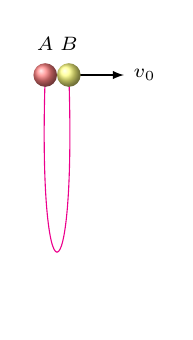
\begin{tikzpicture}[font=\scriptsize]
	\draw[magenta] (0,0)..controls(-.1,-3)and(.4,-3)..(.3,0);
	\draw[-latex] (.3,0)--(1,0)node[right]{\(v_0\)};
	\shade[ball color=red!50] (0,0) circle(.15);
	\shade[ball color=yellow!50] (.3,0) circle(.15);
	\node at(0,.4){\(A\)};
	\node at(.3,.4){\(B\)};
\end{tikzpicture}
\begin{answer}
	（1）\(\frac{1}{2}mv_0\)（2）\(\frac{1}{4}mv_0^2\)（3）\(2mg(\frac{L}{v_0} - 2t_0)\)（3）\(L + 0.6v_0t_0\)\qquad 提示：
\end{answer}